\documentclass{beamer}

\usepackage{graphicx}

\begin{document}
%=============================================================================%
%- https://epilab.ich.ucl.ac.uk/coursematerial/statistics/summarising_normal_dist/non_normal/transformations.html
%=============================================================================%
\begin{frame}
\textbf{Transformations of Non-Normal Data} 
\Large
\begin{itemize}
\item Sometimes non-normally distributed data can be transformed to normality.

\item \textbf{Important:} The transformations used should not change the relative ordering of the values but \textbf{alter the distance between successively ordered values }to change the overall shape of the distribution.

\item For example, if a dataset is transformed by squaring each of the values the larger values will be pulled further apart than the smaller values.
\end{itemize}

\end{frame}
%%=============================================================================%
%\begin{frame}
%. To illustrate:
%\end{frame}
%%=============================================================================%
%\begin{frame}
%\textbf{Transformations of Non-Normal Data} 
%\Large
%	\begin{itemize}
%\item There is a difference of 1 between the values 2 and 3 prior to transformation.
%\item after squaring the measurements 2 becomes 4 and 3 becomes 9 
%\item the difference between the transformed measures is 5 (9-4).
%\item There is a difference of 1 between 10 and 11 prior to transformation; after squaring the measurements 10 becomes 100 and 11 becomes 121 and the difference between the transformed measures is 21 (=121-100)
%and hence after transformation the higher measurements (10 and 11) are more apart than the smaller (2 and 3).
%	\end{itemize}
%
%\end{frame}
%%=============================================================================%
%\begin{frame}
%Squaring data values can therefore be used to normalise downward skew data (by pulling apart the higher measurements an upward tail is created to match the downward skew and hence give a normal distribution).
%\end{frame}
%=============================================================================%
\begin{frame}
	\large
\textbf{Choosing Your Transformation Method}
\begin{itemize}
\item There are a variety of transformations that can be used to correct for skewing to a greater or lesser extent. The correct transformation to use will depend on both the direction and extent of skew. 
\item \textbf{Important} - It is possible to over-correct by using too powerful a transformation and change the direction of the skew. \item For example, a small amount of downward skewing might be over-balanced by squaring the measurements and result in an upward skew distribution.
	\end{itemize}

\end{frame}
%=============================================================================%
\begin{frame}
\textbf{Skewness}
	\begin{figure}
\centering
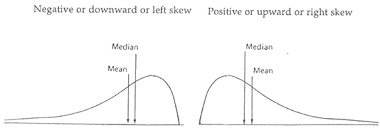
\includegraphics[width=0.99\linewidth]{images/Skew}

\end{figure}

\end{frame}
%=============================================================================%
\begin{frame}
\frametitle{Tukey's Ladder}
\Large
Tukeys ladder of transformations (shown below) gives several common transformations to correct skew in each direction and illustrates the relative effectiveness of these.

\begin{figure}
\centering
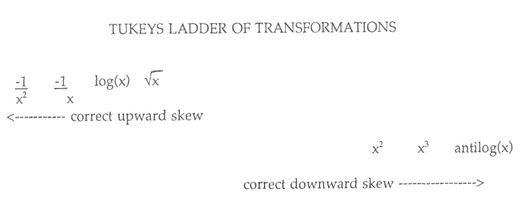
\includegraphics[width=1.10\linewidth]{images/TukeyLadder}
\end{figure}

\end{frame}
%=============================================================================%
\begin{frame}
	\frametitle{Tukey's Ladder}
	\Large
	\vspace{-1cm}
\begin{itemize}
\item For example, the ladder shows that squaring corrects downward skew and that cubing the data gives an even stronger correction. 
\item If we cube rather than square the values then the right hand (higher) values are pulled apart even more, creating a more extreme upper tail.
\end{itemize}
\bigskip
\textit{(Remark from last slide - Antilogging essentially is getting the exponential of a number)}
\end{frame}
%=============================================================================%
\begin{frame}
\frametitle{Tukey's Ladder}
	\Large
\begin{itemize}
\item Upwardly skew data is not uncommon in medical applications and many measurements which display upward skewing are what is known as \textbf{lognormally distributed}. 
\item When data is lognormally distributed, taking logarithms (or logs) of the data values will normalise the data.
\end{itemize}
\end{frame}
%=============================================================================%
\begin{frame}
	\textbf{The Log-Normal distribution}
	\begin{figure}
\centering
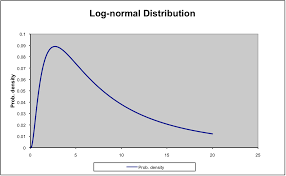
\includegraphics[width=0.99\linewidth]{images/lognormall}
\end{figure}

\end{frame}
%=============================================================================%
\begin{frame}
Example: Serum triglyceride values in cord-blood are lognormal :-
	\\ \textbf{Before Log Transformation}\\
\begin{figure}
\centering
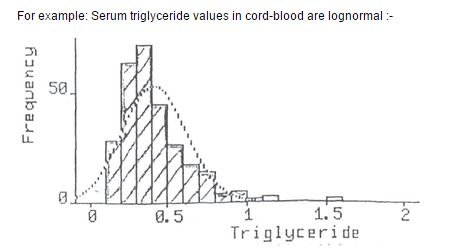
\includegraphics[width=0.9\linewidth]{images/logTransform1}

\end{figure}



\end{frame}
%=============================================================================%
\begin{frame}
	Example: Serum triglyceride values in cord-blood are lognormal :-
	\\ \textbf{After Log Transformation}\\
	\begin{figure}
		\centering
		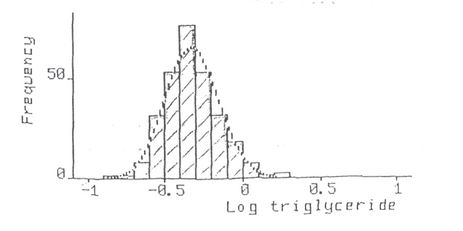
\includegraphics[width=0.9\linewidth]{images/logTransform2}
	\end{figure}	
	
\end{frame}
%=============================================================================%
\begin{frame}
	\Large
	\textbf{Choosing Your Transformation Method}
\begin{itemize}
\item \textbf{Important: }Choosing a suitable transformation can be a matter of trial and error.  \bigskip
\item \textbf{Important: }Transformation may not necessarily work.  \bigskip
\item Log-Transformation corrects upward skewness, if data is downwardly skew then logging will make the skewness worse. \bigskip
\item Downward skew may be corrected (to varying extents) by squaring, cubing or computing the exponential (anti-logging).
\end{itemize}

\end{frame}
%=============================================================================%
\begin{frame}
	\Large
	\textbf{Choosing Your Transformation Method}
	\begin{itemize}
\item Often it is possible to use a transformation that has some biological basis. \bigskip
\item For example, taking square roots of areas or cube roots of volumes may be effective.  \bigskip
\item Taking logarithms may not seem intuitive but this transformation is particularly useful when there are different groups to be transformed and compared. 
	\end{itemize}
% The particular properties of logarithmic transformation are illustrated later in this course.
\end{frame}
%=============================================================================%
\begin{frame}
	\large
	\vspace{-0.8cm}
\textbf{Review}
\begin{itemize}
	\item Describe the purpose of transformations
	\item Describe the process of transformations
	\item Describe the purpose of Tukey's Ladder (referencing direction and relative strength)
	\item Give an example of a transformation for various types of skewed data (use Tukey's Ladder, with an example for both directions)
	\item Describe the limitations of transformations
	\end{itemize}	
\bigskip
\textbf{Remark}: Box-Cox transformations are omitted from the course, but I would still like you to be familiar with the name, and that is related to this topic.
	\end{frame}

%=============================================================================%
\end{document}